\section{Building a Benchmark with Known Truth}
\label{sec:benchmark}

\subsection{What a benchmark needs}
\label{sec:benchmark-needs}

For a real planet the true spectrum is unknown. An injection test supplies a
truth: a known transmission spectrum is added to detector data, and the
spectrum that each method recovers is compared with it.
Section~\ref{sec:validation-problem} listed what such a test needs for SOSS: a
real exposure, a measured image of the star, injection into the raw reads,
and several pipelines that run without knowing the truth. The image of the star matters because only starlight dims during a
transit, so the injector has to decide which of the observed light is
starlight. If it decides this with the same kind of model that a pipeline uses
to separate starlight from background, the errors of that model are hidden and
the pipeline is favoured, a problem known as an inverse crime
\citep{KaipioSomersalo2007}. A measured image of the star avoids this
particular risk. My first
injectors were built from the WASP-17~b data alone, and this section describes
what they taught me.

\subsection{Injecting into the raw reads}
\label{sec:raw-injection}

My first injector added the transit to the count-rate images, after the
detector stages that fit the ramps. This is simple, but it adds the transit
only after the steps in which each pipeline processes the data in its own
way. To make the test fair to every pipeline, I therefore moved the injection
to the raw reads, so that each pipeline runs all of its own steps on the
injected data.

On the same data, NOVA's root-mean-square error for the reference atmosphere
then rose from 125 to 182~ppm, and its spectrum was about 90~ppm too deep. The main reason was the correction of the $1/f$ noise
(Section~\ref{sec:detector-to-spectrum}). In each column, this correction
estimates the stripe from the light left in the pixels outside the traces
after a median out-of-transit image has been subtracted. In exoTEDRF, whose
correction NOVA also uses (Section~\ref{sec:detector-processing}), this
median image is scaled by the measured light curve, so that it dims during the
transit.

My injector, however, dimmed only its model of the star. Near the traces, this model matched the real images, but outside them, at 0.85 to $1.75\,\mu\mathrm{m}$ in order~1, it held only about a third of the light that the correction expects to dim. In the real data, the dimming there was consistent with what the correction assumes, so much of this faint light seems to behave like starlight. During the transit, the correction therefore found too
much light left outside the traces, mistook it for $1/f$ noise and removed it
from the whole column, so the transit became about 1 to 2\% too deep. To
confirm this, I subtracted from the injected data the $1/f$ correction
calculated from the same data without the transit. There, the light curve is
flat, so the correction removes the same stripes but has no transit to react
to. NOVA's error then fell to 150~ppm, so the correction caused about half of
the increase.

How much of the faint light outside the traces dims therefore matters.
To inject a transit correctly, I would need to know how much of the light is
starlight, near the traces, in their wings and far from them, and dim exactly
that.

\subsection{Which light belongs to the star}
\label{sec:which-light}

The WASP-17~b data alone cannot say how much of this light is starlight, not
even inside the extraction box. To see how much this matters, I made three
injections. All three dim the measured light in the wings, 16 to 80 pixels
from the traces. The lower estimate counts as starlight near the traces only
the light explained by a model of the star. I made this model by fitting the
star's spectrum, with a slow change in time, to the out-of-transit images
through ATOCA's model of the detector, together with a smooth background made
of four of NOVA's eight background maps and held in place by the same
off-trace pixels (Section~\ref{sec:continuum}). In exoTEDRF's 40-row extraction box, this estimate leaves typically 0.4, 2.2 and 4.0\% of the light undimmed at 1.0 to 1.8, 1.8 to 2.3 and 2.3 to $2.8\,\mu\mathrm{m}$. The lower estimate also leaves the faint light beyond 80
pixels undimmed. The second injection is the same, except that it also dims
this faint light; it changed NOVA's spectrum by about 40~ppm. The upper
estimate instead counts all the light in the box as starlight and dims it,
and leaves the faint light beyond 80 pixels undimmed, like the lower estimate.

\begin{figure}[t]
  \centering
  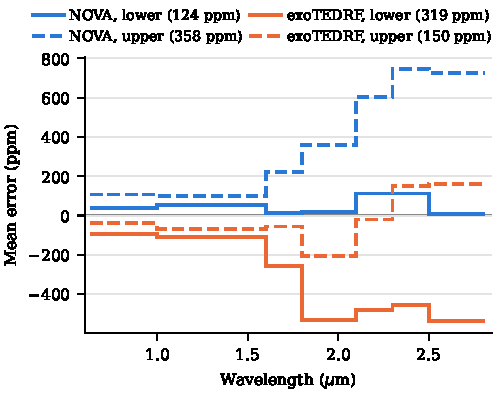
\includegraphics[width=\columnwidth]{figures/benchmark_flip_regional_errors.pdf}
  \caption{Mean error of the spectra recovered by \nova{} (blue) and exoTEDRF
  (orange) from the reference atmosphere injected into the WASP-17~b data, in
  seven wavelength regions, under the lower (solid) and upper (dashed)
  estimates of the starlight. The error is the recovered minus the injected
  depth, so a positive value means that the recovered transit is too deep. The
  legend gives the root-mean-square error in ppm over the 147 reporting bins
  of Section~\ref{sec:transit}.
  Both pipelines reduced raw data made with the same injection recipe, each
  with its own processing.}
  \label{fig:flip}
\end{figure}

Under the lower estimate, NOVA recovered the reference atmosphere with an
error of 124~ppm and exoTEDRF with 319~ppm. Under the upper estimate the order
reversed, with 358~ppm for NOVA and 150~ppm for exoTEDRF
(Figure~\ref{fig:flip}). Each pipeline did best under the estimate that matches
how it treats the faint light. exoTEDRF counts all the light left in its box
after background subtraction as starlight, like the upper estimate, whereas
the lower estimate split the light much as NOVA does, with part of NOVA's own
background model.

Neither estimate is the truth. The upper estimate assumes that all the light
in the box is starlight, which may not be so. The lower estimate depends on
how its fit split the light between the star and a smooth background, a split
that the out-of-transit data could not determine. Between the two estimates,
both pipelines' errors changed by about 500~ppm in the red, so a benchmark
built from the WASP-17~b data alone cannot say which method is more accurate.

\subsection{The real data cannot decide}
\label{sec:real-data-test}

I also tried to measure the share of starlight directly from the real data.
If the bright centre of the trace is almost pure starlight, and all the light in the extraction box is starlight too, the box dims during the transit by the same fraction as the centre; if part of it is background, the box dims less. In the red part of order~1, the two typically agreed to within about 1\%, which would favour the upper estimate. To check how reliable this comparison is, I
repeated it on stretches without a transit: I fitted the same transit shape,
at a time when no transit happens, to the box and to the bright centre. Both
fitted depths should be zero. Instead, they differed by up to about 11\% of the
real transit depth, ten times more than the 1\% needed to tell the two
estimates apart. The real data therefore cannot decide.

I also measured how much the faint light outside the traces dims during the real transit, on the pixels that the $1/f$ correction uses. At 0.85 to $1.75\,\mu\mathrm{m}$ in order~1, it dimmed by $0.033\pm0.007$~DN\,s$^{-1}$ per pixel, as much as if all the light left there after background subtraction were starlight. This suggests that most of this light behaves like starlight, but it cannot tell the injector how much of it to dim. Only this range gives a clear answer: at 1.75 to $2.1\,\mu\mathrm{m}$ the measurement is too noisy to tell the cases apart, and at 2.1 to $2.8\,\mu\mathrm{m}$ the light appears to dim about four times more than even starlight would, which I cannot explain. Even where the answer is clear, it depends on how the detector behaves: if the fit allows the detector's level to change during the transit, the share of this light that dims like starlight ranges from about half to all of it.

Separating starlight
from background needs extra information, such as exposures in which the star
sits elsewhere on the detector. Such exposures are the basis of the benchmark
in the next section.
